\ifdefined\inMainDoc\else
\documentclass[12pt,a4paper]{article}
% ================================================================
%  PRÉAMBULE COMMUN - ANNALES CORRIGÉES
%  Université de Kara - FaST - Licence Fondamentale MPC
%  Design optimisé impression noir et blanc
% ================================================================

% -- ENCODAGE & LANGUE --
\usepackage[utf8]{inputenc}
\usepackage[T1]{fontenc}
\usepackage[french]{babel}
\usepackage{lmodern}
\usepackage{microtype}

% -- MISE EN PAGE --
\usepackage[a4paper, top=2.8cm, bottom=2.5cm, left=2.5cm, right=2.5cm, headheight=14pt]{geometry}
\usepackage{setspace}
\setstretch{1.2}
\usepackage{parskip}
\setlength{\parindent}{1.2em}
\setlength{\parskip}{4pt}

% -- MATHS --
\usepackage{amsmath, amssymb, mathtools, amsthm}
\usepackage{mathrsfs}
\usepackage{dsfont}
\usepackage{bm}
\usepackage{cancel}
\usepackage{textcomp}
% Définition de \oiint (intégrale de surface fermée) sans package supplémentaire
\newcommand{\oiint}{\mathop{\iint\!\!\!\!\!\!\!\bigcirc}\limits}

% -- PHYSIQUE & CHIMIE --
\usepackage{physics}
\usepackage{siunitx}
% Lorsque physics est chargé, siunitx omet \qty. On le restaure ici :
\AtBeginDocument{\RenewCommandCopy\qty\SI}
\sisetup{locale = FR, detect-all, output-decimal-marker={,}}
% Commande de substitution pour les unités posant problème avec pdflatex
% (ohm, degreeCelsius, micro, angstrom, percent utilisent des caractères non-ASCII)
\newcommand{\qtyohm}[1]{\ensuremath{\num{#1}\,\Omega}}
\newcommand{\qtydegc}[1]{\ensuremath{\num{#1}\,{}^\circ\text{C}}}
\newcommand{\qtyangstrom}[1]{\ensuremath{\num{#1}\,\text{\AA}}}
\newcommand{\qtypercent}[1]{\ensuremath{\num{#1}\,\%}}
\newcommand{\qtyum}[1]{\ensuremath{\num{#1}\,\mu\text{m}}}
\usepackage[version=4]{mhchem}

% -- GRAPHISMES --
\usepackage{graphicx}
\usepackage{float}
\usepackage{caption}
\usepackage{subcaption}
\usepackage{wrapfig}
\usepackage{tikz}
\usetikzlibrary{calc, arrows.meta, patterns, shapes.geometric}
\usepackage{pgfplots}
\pgfplotsset{compat=1.18}

% -- TABLEAUX --
\usepackage{booktabs}
\usepackage{array}
\usepackage{tabularx}
\usepackage{multirow}

% -- LISTES --
\usepackage{enumitem}
\setlist[enumerate]{topsep=3pt, itemsep=2pt, parsep=0pt}
\setlist[itemize]{topsep=3pt, itemsep=2pt, parsep=0pt, label={.}}

% -- BOÎTES (noir et blanc) --
\usepackage{mdframed}
\usepackage{tcolorbox}
\tcbuselibrary{skins, breakable, theorems}

% Boîte EXERCICE : encadré avec filet épais, fond blanc
\newmdenv[
  linewidth=1.2pt,
  linecolor=black,
  roundcorner=3pt,
  skipabove=10pt,
  skipbelow=6pt,
  innertopmargin=8pt,
  innerbottommargin=8pt,
  innerleftmargin=10pt,
  innerrightmargin=10pt,
  backgroundcolor=white,
  frametitle={\bfseries\small Exercice},
  frametitlealignment=\raggedright,
  frametitleaboveskip=4pt,
  frametitlebelowskip=4pt,
]{boiteexercice}

% Boîte CORRIGÉ : fond gris très clair + filet fin
\newmdenv[
  linewidth=0.6pt,
  linecolor=black,
  leftline=true,
  rightline=false,
  topline=false,
  bottomline=false,
  linecolor=black,
  innerleftmargin=12pt,
  innerrightmargin=8pt,
  innertopmargin=6pt,
  innerbottommargin=6pt,
  backgroundcolor=gray!8,
  skipabove=4pt,
  skipbelow=8pt,
]{boitecorrige}

% Boîte RÉSUMÉ DE COURS : double encadré
\newmdenv[
  linewidth=0.8pt,
  linecolor=black,
  roundcorner=2pt,
  backgroundcolor=gray!12,
  innertopmargin=10pt,
  innerbottommargin=10pt,
  innerleftmargin=12pt,
  innerrightmargin=12pt,
  skipabove=12pt,
  skipbelow=8pt,
]{boiteresume}

% Boîte ATTENTION/REMARQUE : barre gauche épaisse
\newmdenv[
  leftline=true,
  rightline=false,
  topline=false,
  bottomline=false,
  linewidth=3pt,
  linecolor=black,
  backgroundcolor=gray!5,
  innerleftmargin=12pt,
  innerrightmargin=8pt,
  innertopmargin=5pt,
  innerbottommargin=5pt,
  skipabove=6pt,
  skipbelow=6pt,
]{boiteremarque}

% -- DIFFICULTÉ DES EXERCICES --
\newcommand{\facile}{$\star$}
\newcommand{\moyen}{$\star\!\star$}
\newcommand{\difficile}{$\star\!\star\!\star$}
\newcommand{\niveau}[1]{\hfill\textbf{#1}\hspace{2pt}}

% -- EN-TÊTES ET PIEDS DE PAGE --
\usepackage{fancyhdr}
\pagestyle{fancy}
\fancyhf{}
\renewcommand{\headrulewidth}{0.5pt}
\renewcommand{\footrulewidth}{0.3pt}

% -- HYPERLIENS --
\usepackage[hidelinks]{hyperref}
\hypersetup{
    colorlinks=false,
    pdftitle={Annale Corrigée - Licence MPC - Université de Kara}
}

% -- TITRES --
\usepackage{titlesec}
\titleformat{\section}{\Large\bfseries}{\thesection.}{0.8em}{}[\vspace{2pt}\hrule\vspace{4pt}]
\titleformat{\subsection}{\large\bfseries}{\thesubsection.}{0.7em}{}
\titleformat{\subsubsection}{\normalsize\bfseries}{\thesubsubsection.}{0.6em}{}

% -- THÉORÈMES --
\theoremstyle{definition}
\newtheorem{defn}{Définition}[section]
\newtheorem{prop}{Propriété}[section]
\newtheorem{thm}{Théorème}[section]
\newtheorem{corol}{Corollaire}[section]
\newtheorem{exemple}{Exemple}[section]

% -- COMMANDES MATHÉMATIQUES UTILES --
\newcommand{\vect}[1]{\overrightarrow{#1}}
\newcommand{\R}{\mathbb{R}}
\newcommand{\N}{\mathbb{N}}
\newcommand{\Z}{\mathbb{Z}}
\newcommand{\C}{\mathbb{C}}
\renewcommand{\d}{\mathrm{d}}
\newcommand{\deriv}[2]{\dfrac{\d #1}{\d #2}}
\newcommand{\dpart}[2]{\dfrac{\partial #1}{\partial #2}}
\newcommand{\rot}{\overrightarrow{\mathrm{rot}}\,}
\renewcommand{\div}{\mathrm{div}\,}
\renewcommand{\grad}{\overrightarrow{\mathrm{grad}}\,}
\newcommand{\e}{\mathrm{e}}
\newcommand{\ii}{\mathrm{i}}
\renewcommand{\Tr}{\mathrm{Tr}}

% Numérotation des équations par section
\numberwithin{equation}{section}

% -- RÉSULTATS ENCADRÉS --
\newcommand{\res}[1]{\[\boxed{#1}\]}

% -- REMARQUE INLINE --
\newcommand{\rmq}[1]{\begin{boiteremarque}\textbf{Remarque.} #1\end{boiteremarque}}

% -- MISE EN VALEUR DU RÉSULTAT FINAL --
\newcommand{\reponse}[1]{%
  \begin{center}
    \fbox{\begin{minipage}{0.92\textwidth}\centering #1\end{minipage}}
  \end{center}%
}


% En-têtes et pieds de page
\lhead{\textbf{Mécanique du Solide} - Licence 2}
\rhead{Université de Kara - FaST}
\cfoot{\thepage}
\lfoot{\textit{Licence Fondamentale MPC}}
\rfoot{\textit{Annales corrigées}}

\begin{document}
\fi

\begin{center}
  {\LARGE\bfseries Mécanique du Solide}\\[6pt]
  {\large Licence 2 - Mathématiques, Physique, Chimie}\\[4pt]
  {\normalsize Université de Kara - Faculté des Sciences et Techniques}
\end{center}

\vspace{8pt}
\hrule
\vspace{12pt}

% ================================================================
\section{Résumé de cours}
% ================================================================

\begin{boiteresume}
\textbf{1. Torseurs et cinématique du solide}

Un torseur $[T]$ est défini par sa résultante $\vec{R}$ et son moment $\vec{M}_A$ en un point $A$. La loi de transport est :
\[
\vec{M}_B = \vec{M}_A + \overrightarrow{BA} \wedge \vec{R}.
\]

Le \textbf{torseur cinématique} d'un solide $(S)$ par rapport à un repère $(R)$ a pour résultante le vecteur rotation instantané $\vec{\Omega}(S/R)$ et pour moment en $A$ la vitesse $\vec{V}(A \in S/R)$.

Pour deux solides $(S_1)$ et $(S_2)$ et un repère intermédiaire $(R_1)$ :
\[
\vec{\Omega}(S_2/R) = \vec{\Omega}(S_2/R_1) + \vec{\Omega}(R_1/R).
\]

Vitesse d'un point $B$ du solide connaissant la vitesse de $A$ :
\[
\vec{V}(B \in S/R) = \vec{V}(A \in S/R) + \vec{\Omega}(S/R) \wedge \overrightarrow{AB}.
\]

\medskip
\textbf{2. Centre de masse}

\[
\overrightarrow{OG} = \frac{1}{M}\int \overrightarrow{OM}\,\mathrm{d}m, \qquad M = \int \mathrm{d}m.
\]
Pour un système discret : $\overrightarrow{OG} = \dfrac{1}{M}\sum m_i\,\overrightarrow{OM_i}$.

\medskip
\textbf{3. Moment d'inertie - Théorème de Huygens-Steiner}

Le moment d'inertie d'un solide par rapport à un axe $\Delta$ passant par $G$ vaut $I_G$. Par rapport à un axe $\Delta'$ parallèle à $\Delta$ et distant de $d$ :
\[
I_{\Delta'} = I_G + M\,d^2.
\]

Moments d'inertie usuels (solide de masse $M$) :
\begin{itemize}
  \item Tige de longueur $2\ell$ par rapport au centre : $I_G = \dfrac{M\ell^2}{3}$.
  \item Disque de rayon $R$ par rapport à son axe : $I = \dfrac{MR^2}{2}$.
  \item Sphère pleine de rayon $R$ par rapport à un diamètre : $I = \dfrac{2MR^2}{5}$.
\end{itemize}

\medskip
\textbf{4. Théorème du moment cinétique pour un solide}

Le moment cinétique en $G$ : $\vec{\sigma}(G, S/R) = [I_G]\,\vec{\Omega}(S/R)$ (avec $[I_G]$ tenseur d'inertie).

Pour un mouvement de rotation autour d'un axe fixe $\Delta$ :
\[
\frac{\mathrm{d}}{\mathrm{d}t}\bigl(I_\Delta\,\dot{\theta}\bigr) = \sum \mathcal{M}_\Delta(\vec{F}_{\mathrm{ext}}).
\]

\medskip
\textbf{5. Énergie cinétique - Théorème de Koenig}

\[
E_c(S/R) = \frac{1}{2}M\,\vec{V}^2(G/R) + \frac{1}{2}I_G\,\omega^2 \quad \text{(mouvement plan).}
\]

Plus généralement : $E_c = \dfrac{1}{2}M V_G^2 + \dfrac{1}{2}\vec{\Omega}\cdot\vec{\sigma}(G)$.

Le théorème de l'énergie cinétique : $\dfrac{\mathrm{d}E_c}{\mathrm{d}t} = \mathcal{P}(\vec{F}_{\mathrm{ext}})$.

\medskip
\textbf{6. Liaisons mécaniques courantes}

\begin{itemize}
  \item \textbf{Pivot} (axe $z$) : un seul degré de liberté en rotation $\dot{\theta}$.
  \item \textbf{Glissière} (axe $x$) : un seul degré de liberté en translation $\dot{x}$.
  \item \textbf{Pivot-glissant} (axe $z$) : rotation $\dot{\theta}$ et translation $\dot{z}$ autour et le long du même axe.
  \item \textbf{Rotule} : 3 degrés de liberté en rotation, aucune translation.
\end{itemize}

\medskip
\textbf{7. Équilibre d'un solide - Conditions de Dirichlet}

Un solide est en équilibre si et seulement si la résultante et le moment résultant de toutes les forces extérieures sont nuls :
\[
\sum \vec{F}_i = \vec{0}, \qquad \sum \vec{M}_A(\vec{F}_i) = \vec{0}.
\]
\end{boiteresume}

% ================================================================
\section{Exercices corrigés}
% ================================================================

% ----------------------
\begin{boiteexercice}
\textbf{Exercice 1 - Application antisymétrique et vecteur de rotation}\niveau{\moyen}

Soit $L$ une application de l'espace vectoriel $E$ dans lui-même, définie par :
\[
L(\vec{u}) = \begin{pmatrix} \beta x - y + 4z \\ x + \beta y + \gamma z \\ -\alpha^2 x - y + \beta z \end{pmatrix}
\quad \text{avec } \vec{u} = \begin{pmatrix} x \\ y \\ z \end{pmatrix}.
\]
\begin{enumerate}
  \item Pour quelles valeurs de $\alpha$, $\beta$, $\gamma$ l'application $L$ est-elle antisymétrique ?
  \item Montrer qu'il existe un vecteur $\vec{\Omega}$ tel que $L(\vec{u}) = \vec{\Omega} \wedge \vec{u}$, et déterminer $\vec{\Omega}$.
\end{enumerate}
\end{boiteexercice}

\begin{boitecorrige}
\textbf{1.} $L$ est antisymétrique si et seulement si sa matrice $\mathbf{L}$ vérifie $\mathbf{L}^T = -\mathbf{L}$, ce qui impose des éléments diagonaux nuls et une antisymétrie des éléments hors diagonaux.

La matrice associée à $L$ dans la base $(\vec{i}, \vec{j}, \vec{k})$ est :
\[
\mathbf{L} = \begin{pmatrix} \beta & -1 & 4 \\ 1 & \beta & \gamma \\ -\alpha^2 & -1 & \beta \end{pmatrix}.
\]

Condition $\mathbf{L}^T = -\mathbf{L}$ :
\[
\begin{cases} \beta = 0 & \text{(diagonale nulle)} \\ \gamma + 4 = 0 \Rightarrow \gamma = -4 & (\text{mais on lit ici : vérification ligne par ligne}) \end{cases}
\]

Plus précisément, $L_{12} = -1$ et $L_{21} = 1$ donnent bien $L_{12} = -L_{21}$ : condition satisfaite. $L_{13} = 4$ et $L_{31} = -\alpha^2$ donnent $-\alpha^2 = -4$, soit $\alpha^2 = 4$, c'est-à-dire $\alpha = \pm 2$. $L_{23} = \gamma$ et $L_{32} = -1$ donnent $\gamma = 1$. La diagonale impose $\beta = 0$.

Ainsi : $\beta = 0$, $\gamma = 1$, $\alpha = \pm 2$, et :
\[
\mathbf{L} = \begin{pmatrix} 0 & -1 & 4 \\ 1 & 0 & 1 \\ -4 & -1 & 0 \end{pmatrix}.
\]

\textbf{2.} Pour une matrice antisymétrique $3 \times 3$, il existe toujours $\vec{\Omega} = (a, b, c)^T$ tel que $L(\vec{u}) = \vec{\Omega} \wedge \vec{u}$.

\[
\vec{\Omega} \wedge \vec{u} = \begin{pmatrix} bz - cy \\ cx - az \\ ay - bx \end{pmatrix}.
\]

En identifiant avec $L(\vec{u}) = \begin{pmatrix} -y + 4z \\ x + z \\ -4x - y \end{pmatrix}$, on obtient :
\[
\begin{cases} b = 4, \quad c = 1 \\ c = 1, \quad a = -1 \\ a = -1, \quad b = 4 \end{cases}
\quad \Rightarrow \quad \vec{\Omega} = \begin{pmatrix} -1 \\ 4 \\ 1 \end{pmatrix}.
\]

\begin{center}
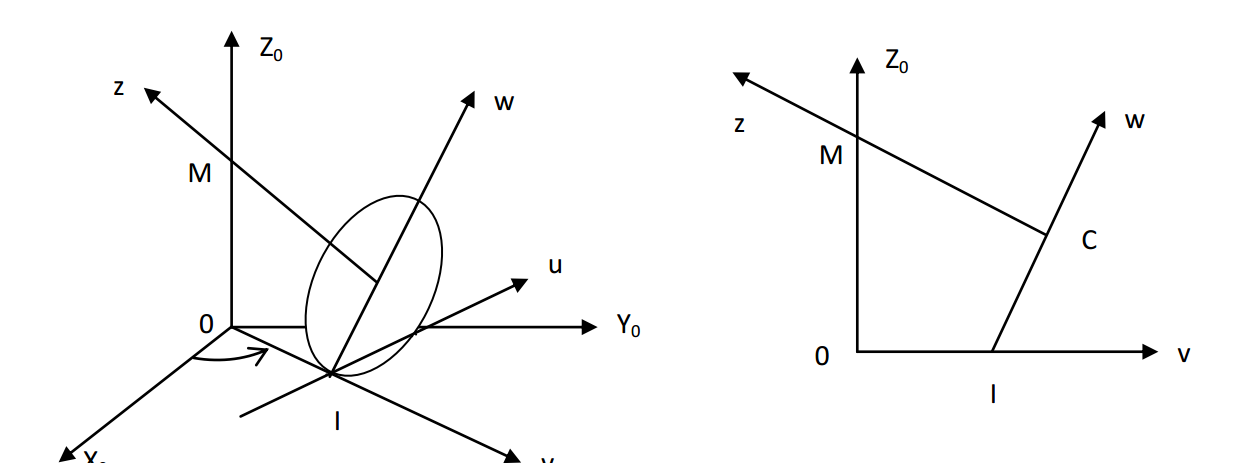
\includegraphics[width=0.45\textwidth]{images/mecanique_solide/ms-006-004.png}\\[4pt]
{\small\itshape Application linéaire antisymétrique $L(\vec{u}) = \vec{\Omega}\wedge\vec{u}$ : repérage du vecteur rotation $\vec{\Omega}$.}
\end{center}
\end{boitecorrige}

% ----------------------
\begin{boiteexercice}
\textbf{Exercice 2 - Torseurs cinématiques : disque en rotation}\niveau{\facile}

Dans un repère $R(O, \vec{i}, \vec{j}, \vec{k})$, un disque de centre $O$ contenu dans le plan $xOy$ tourne dans le sens trigonométrique autour de $Oz$ avec une vitesse angulaire $\omega$.

\begin{enumerate}
  \item Déterminer la vitesse $\vec{V}(M/R)$ d'un point $M(x, y, 0)$ du disque.
  \item Montrer que le champ $\vec{V}(M/R)$ est un torseur et en déterminer les éléments de réduction en $O$.
  \item De quel type de torseur s'agit-il ? Quel est son axe central ?
\end{enumerate}
\end{boiteexercice}

\begin{boitecorrige}
\textbf{1.} Le vecteur rotation du disque est $\vec{\Omega} = \omega\,\vec{k}$. La vitesse de $M$ est :
\[
\vec{V}(M/R) = \vec{\Omega} \wedge \overrightarrow{OM} = \omega\vec{k} \wedge (x\vec{i}+y\vec{j}) = \omega(-y\vec{i} + x\vec{j}).
\]

\textbf{2.} Vérifions que le champ est équiprojectif : pour deux points $M$ et $M'$,
\[
\overrightarrow{MM'} \cdot \bigl(\vec{V}(M) - \vec{V}(M')\bigr) = \overrightarrow{MM'} \cdot \bigl[\vec{\Omega} \wedge \overrightarrow{MM'}\bigr] = 0,
\]
car le produit scalaire d'un vecteur par son produit vectoriel avec un autre est nul. Le champ est donc équiprojectif, ce qui en fait un torseur.

Éléments de réduction en $O$ : la résultante est $\vec{R} = \vec{\Omega} = \omega\vec{k}$ et le moment en $O$ est $\vec{V}(O/R) = \vec{0}$.

Les éléments de réduction sont $[V]_O = [\vec{0},\, \omega\vec{k}]$.

\begin{center}
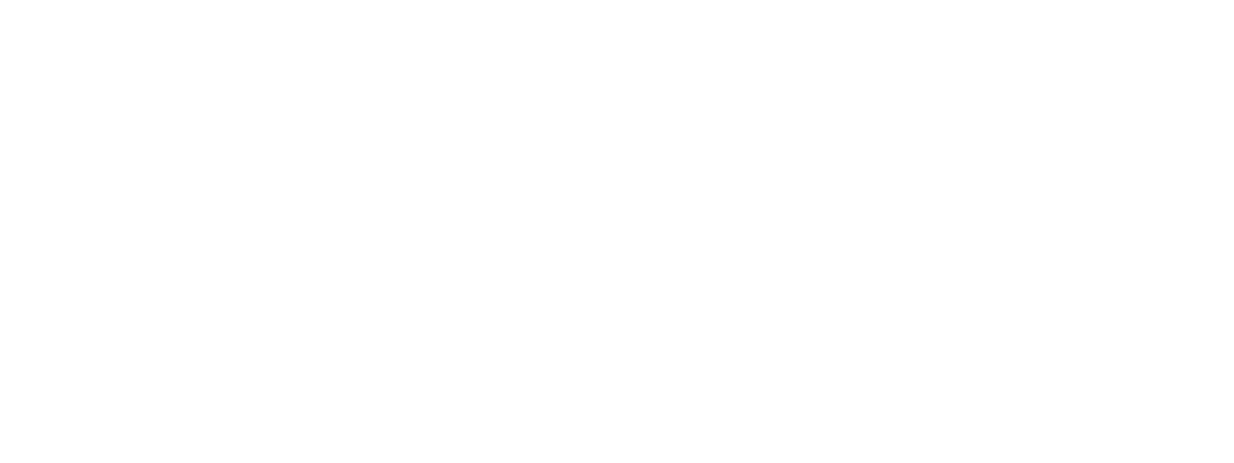
\includegraphics[width=0.45\textwidth]{images/mecanique_solide/ms-006-005.png}\\[4pt]
{\small\itshape Disque en rotation autour de l'axe $Oz$ : vitesse $\vec{V}(M) = \vec{\Omega}\wedge\overrightarrow{OM}$ et équiprojectivité du champ des vitesses.}
\end{center}

\textbf{3.} L'invariant scalaire est $I = \vec{R} \cdot \vec{M}_O = \omega\vec{k} \cdot \vec{0} = 0$. C'est un \textbf{glisseur}. Son axe central est la droite passant par $O$ dirigée selon $\vec{k}$, c'est-à-dire l'axe de rotation $Oz$.
\end{boitecorrige}

% ----------------------
\begin{boiteexercice}
\textbf{Exercice 3 - Centre de masse de solides usuels}\niveau{\moyen}

Déterminer les coordonnées du centre d'inertie $G$ des solides suivants :
\begin{enumerate}
  \item Un arc de cercle homogène de centre $O$, de rayon $R$, de densité linéique $\lambda$, vu sous un angle $2\alpha$ de part et d'autre de l'axe $Ox$.
  \item Une plaque triangulaire homogène de densité surfacique $\sigma$, formant le triangle $OAB$ avec $\overrightarrow{OA} = a\vec{x}$ et $\overrightarrow{OB} = b\vec{y}$.
  \item Une demi-sphère pleine homogène de centre $O$, de rayon $R$, d'axe de symétrie $Oz$, de densité $\rho$.
\end{enumerate}
\end{boiteexercice}

\begin{boitecorrige}
\textbf{1. Arc de cercle.}

Par symétrie par rapport à $Ox$, on a $y_G = z_G = 0$. En paramétrant l'arc par l'angle $\varphi \in [-\alpha, \alpha]$ :
\[
x_G = \frac{\displaystyle\int_{-\alpha}^{\alpha} R\cos\varphi\,\lambda R\,\mathrm{d}\varphi}
           {\displaystyle\int_{-\alpha}^{\alpha} \lambda R\,\mathrm{d}\varphi}
= R\,\frac{\bigl[\sin\varphi\bigr]_{-\alpha}^{\alpha}}{2\alpha}
= R\,\frac{\sin\alpha}{\alpha}.
\]

\begin{center}
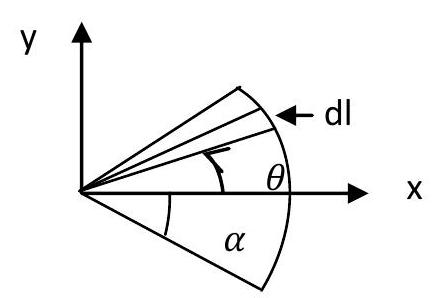
\includegraphics[width=0.45\textwidth]{images/mecanique_solide/ms-008-008.png}\\[4pt]
{\small\itshape Arc de cercle vu sous un angle $2\alpha$ : élément $\mathrm{d}\ell = R\,\mathrm{d}\theta$.}
\end{center}

\textbf{2. Plaque triangulaire.}

La masse totale est $m = \sigma\,\dfrac{ab}{2}$. L'équation de $AB$ est $y = -\dfrac{b}{a}x + b$.

Pour $x_G$ : élément de surface $\mathrm{d}s = y\,\mathrm{d}x$ avec $0 \leq x \leq a$.
\[
x_G = \frac{1}{m}\int_0^a x\sigma y\,\mathrm{d}x = \frac{2\sigma}{ab}\int_0^a x\!\left(-\frac{b}{a}x+b\right)\mathrm{d}x
= \frac{2}{a}\!\left[-\frac{x^3}{3a}+\frac{x^2}{2}\right]_0^a = \frac{2}{a}\cdot\frac{a^2}{6} = \frac{a}{3}.
\]

De même : $y_G = \dfrac{b}{3}$. Le centre de masse du triangle est donc au tiers de chaque côté depuis l'origine.

\begin{center}
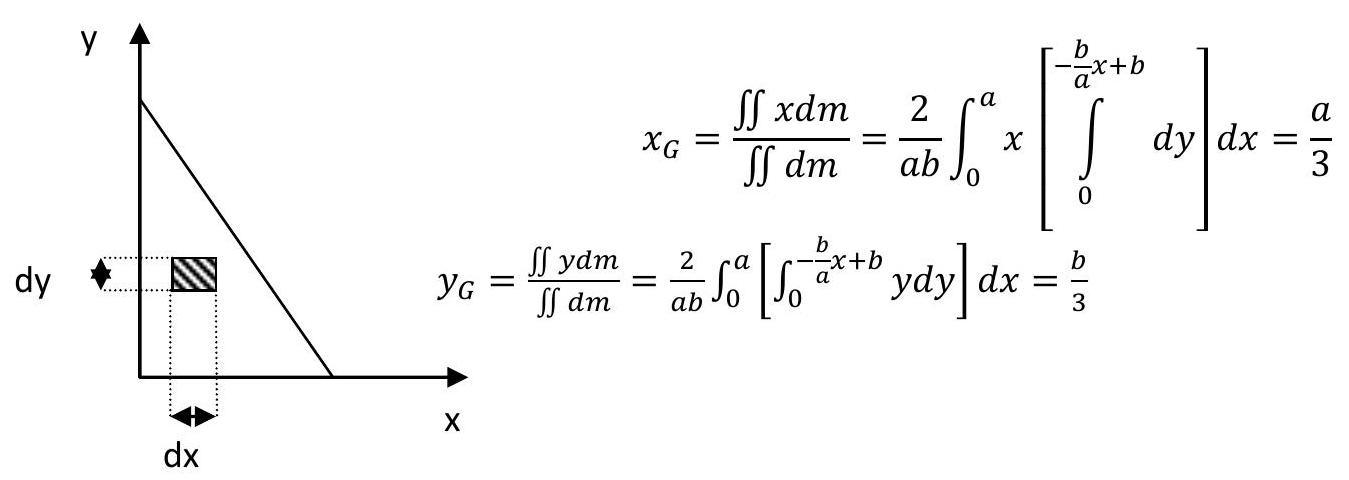
\includegraphics[width=0.45\textwidth]{images/mecanique_solide/ms-009-009.png}\quad
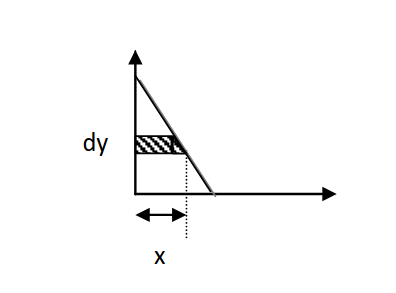
\includegraphics[width=0.40\textwidth]{images/mecanique_solide/ms-009-011.png}\\[4pt]
{\small\itshape Plaque triangulaire : coordonnées du centre de gravité $G(a/3, b/3)$ et élément de surface.}
\end{center}

\begin{center}
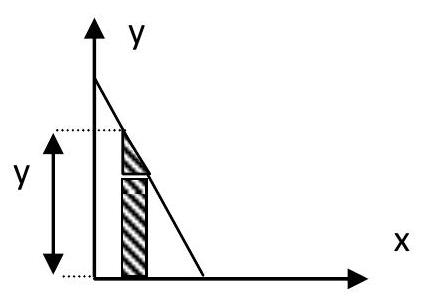
\includegraphics[width=0.45\textwidth]{images/mecanique_solide/ms-009-010.png}\quad
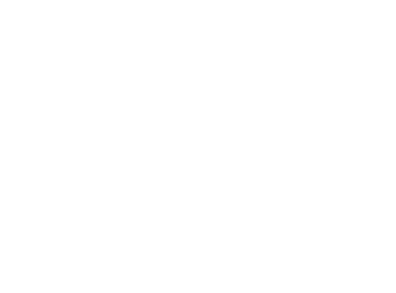
\includegraphics[width=0.40\textwidth]{images/mecanique_solide/ms-009-012.png}\\[4pt]
{\small\itshape Autres vues de la plaque triangulaire : décomposition de l'élément de surface $\d s = y\,\d x$ et intégration sur le domaine $OAB$.}
\end{center}

\textbf{3. Demi-sphère.}

Par symétrie, $x_G = y_G = 0$. En coordonnées sphériques $(r, \theta, \varphi)$ avec $\theta \in [0, \pi/2]$, $r \in [0, R]$ :
\[
z_G = \frac{\displaystyle\int_0^R\!\int_0^{\pi/2}\!\int_0^{2\pi} r\cos\theta \cdot \rho r^2\sin\theta\,\mathrm{d}r\,\mathrm{d}\theta\,\mathrm{d}\varphi}
           {\displaystyle\int_0^R\!\int_0^{\pi/2}\!\int_0^{2\pi} \rho r^2\sin\theta\,\mathrm{d}r\,\mathrm{d}\theta\,\mathrm{d}\varphi}.
\]

Numérateur : $\rho \cdot \dfrac{R^4}{4} \cdot \dfrac{1}{2} \cdot 2\pi = \dfrac{\pi\rho R^4}{4}$.

Dénominateur : $\rho \cdot \dfrac{R^3}{3} \cdot 1 \cdot 2\pi = \dfrac{2\pi\rho R^3}{3}$.

\[
z_G = \frac{\pi\rho R^4/4}{2\pi\rho R^3/3} = \frac{R}{4} \cdot \frac{3}{2} = \frac{3R}{8}.
\]

\begin{center}
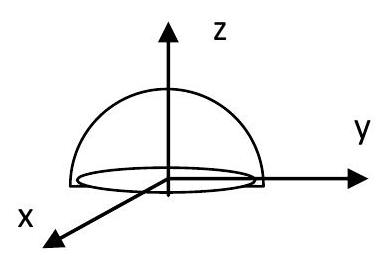
\includegraphics[width=0.40\textwidth]{images/mecanique_solide/ms-010-013.png}\\[4pt]
{\small\itshape Demi-sphère pleine de rayon $R$ : le centre de masse est à $z_G = 3R/8$ de la base.}
\end{center}

\textbf{4. Cône plein (exemple complémentaire).}

Pour un cône droit de hauteur $h$ et de rayon de base $R$, en coordonnées cylindriques :
\[
z_G = \frac{\displaystyle\int_0^h z\,\rho\pi\!\left(R(1-z/h)\right)^2\mathrm{d}z}
           {\displaystyle\int_0^h \rho\pi\!\left(R(1-z/h)\right)^2\mathrm{d}z}
       = \frac{3h}{4}.
\]

\begin{center}
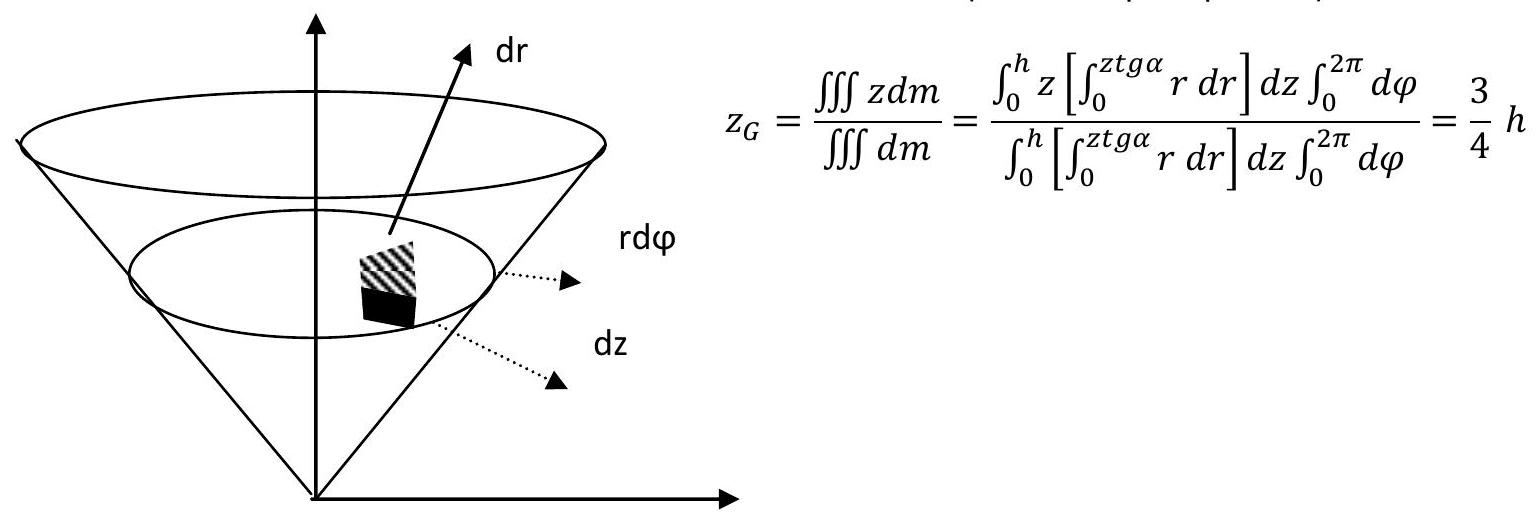
\includegraphics[width=0.40\textwidth]{images/mecanique_solide/ms-010-014.png}\\[4pt]
{\small\itshape Cône de hauteur $h$ : élément de volume et centre de masse $z_G = 3h/4$.}
\end{center}
\end{boitecorrige}

% ----------------------
\begin{boiteexercice}
\textbf{Exercice 4 - Disque sur tapis roulant incliné (dynamique)}\niveau{\difficile}

Un disque homogène de masse $m$, de rayon $r$, de centre $G$, est posé sans vitesse initiale sur un tapis roulant incliné d'un angle $\alpha$ se déplaçant à la vitesse constante $v_0\,\vec{i}_0$ (avec $v_0 > 0$). La réaction de contact est $\vec{R} = T\vec{i}_0 + N\vec{j}_0$ avec $|T| = fN$ tant qu'il y a glissement.

On pose $\overrightarrow{OG} = x_G\vec{i}_0 + r\vec{j}_0$.

\begin{enumerate}
  \item Calculer la vitesse de glissement initiale du disque sur le tapis.
  \item Appliquer le principe fondamental de la dynamique et obtenir les équations du mouvement.
  \item Calculer la dérivée par rapport au temps de la vitesse de glissement.
  \item Décrire l'évolution de la vitesse de glissement selon les valeurs de $f$ et $\alpha$.
\end{enumerate}
\end{boiteexercice}

\begin{boitecorrige}
\textbf{1. Vitesse de glissement initiale.}

\begin{center}
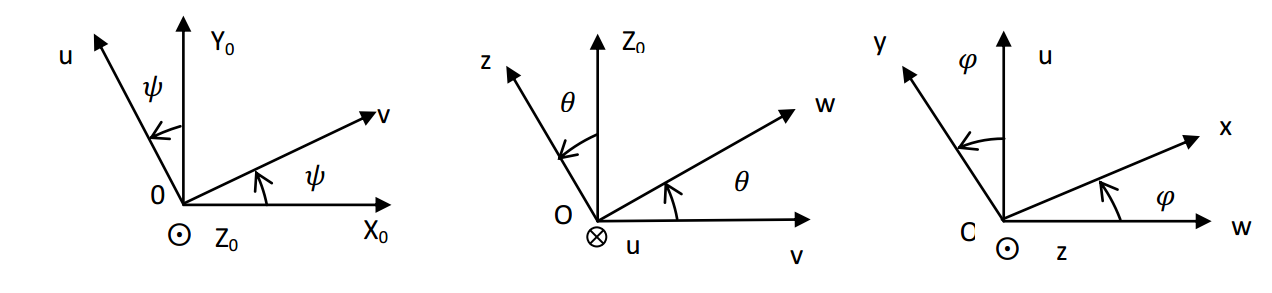
\includegraphics[width=0.50\textwidth]{images/mecanique_solide/ms-006-006.png}\\[4pt]
{\small\itshape Disque posé sur un tapis roulant incliné : repère $(\vec{i}_0, \vec{j}_0)$, angle $\alpha$ et point de contact $I$.}
\end{center}

La vitesse de glissement du disque sur le tapis est :
\[
\vec{v}_g = \vec{V}(I \in S_1/R_0) - \vec{V}(I \in S_2/R_0) = (\dot{x}_G + r\dot{\theta} - v_0)\vec{i}_0.
\]
À $t = 0$, le disque est posé sans vitesse initiale : $\dot{x}_G(0) = 0$, $\dot{\theta}(0) = 0$. Donc :
\[
\vec{v}_{g0} = -v_0\,\vec{i}_0.
\]

\textbf{2. Principe fondamental de la dynamique.}

Théorème de la résultante (projection sur $\vec{i}_0$ et $\vec{j}_0$) :
\[
m\ddot{x}_G = T - mg\sin\alpha, \qquad 0 = N - mg\cos\alpha \Rightarrow N = mg\cos\alpha.
\]

Théorème du moment cinétique en $G$ (moment d'inertie du disque : $I_G = mr^2/2$) :
\[
\frac{mr^2}{2}\,\ddot{\theta} = Tr \quad \Rightarrow \quad \ddot{\theta} = \frac{2T}{mr}.
\]

\textbf{3. Dérivée de la vitesse de glissement.}

\[
\frac{\mathrm{d}v_g}{\mathrm{d}t} = \ddot{x}_G + r\ddot{\theta} = \frac{T}{m} - g\sin\alpha + \frac{2T}{m} = \frac{3T}{m} - g\sin\alpha.
\]

Comme $\vec{v}_{g0} = -v_0\vec{i}_0 < 0$, la force de frottement agit dans le sens de $+\vec{i}_0$ : $T = +fN = fmg\cos\alpha$.

\[
\frac{\mathrm{d}v_g}{\mathrm{d}t} = 3g\cos\alpha\!\left(f - \frac{\tan\alpha}{3}\right).
\]

\textbf{4. Évolution de la vitesse de glissement.}

La vitesse de glissement part de $v_g(0) = -v_0 < 0$.

\begin{itemize}
  \item Si $f > \dfrac{\tan\alpha}{3}$ : $\dfrac{\mathrm{d}v_g}{\mathrm{d}t} > 0$, la vitesse de glissement augmente depuis $-v_0$ jusqu'à $0$. Il y a d'abord glissement, puis roulement pur dès que $v_g = 0$.
  \item Si $f < \dfrac{\tan\alpha}{3}$ : $\dfrac{\mathrm{d}v_g}{\mathrm{d}t} < 0$, la vitesse de glissement décroît à partir de $-v_0$ : il y a toujours glissement.
  \item Si $f = \dfrac{\tan\alpha}{3}$ : la vitesse de glissement reste constante à $-v_0$ ; il y a glissement permanent sans variation.
\end{itemize}
\end{boitecorrige}

% ----------------------
\begin{boiteexercice}
\textbf{Exercice 5 - Roulement d'un cerceau sur un plan}\niveau{\difficile}

Un cerceau $(C_1)$ de rayon $a$, dont le plan est vertical, roule sans glisser sur le plan horizontal $(\pi)$. Le point de contact décrit un cercle de rayon $R$ avec une vitesse angulaire uniforme $\dot{\theta} = \text{cte}$. Soit $R_0(O, \vec{x}_0, \vec{y}_0, \vec{z}_0)$ le repère lié à $(\pi)$ et $R_1(O_1, \vec{x}_1, \vec{y}_1, \vec{z}_0)$ le repère en rotation uniforme autour de $Oz_0$.

\begin{enumerate}
  \item Déterminer $\vec{\Omega}(C_1/R_1)$ et $\vec{\Omega}(C_1/R_0)$.
  \item Calculer les vitesses du point géométrique de contact $I_{G_1}$ et du point matériel $I_1$.
  \item En déduire la condition de roulement sans glissement.
\end{enumerate}
\end{boiteexercice}

\begin{boitecorrige}
\textbf{1. Vecteurs rotation.}

\begin{center}
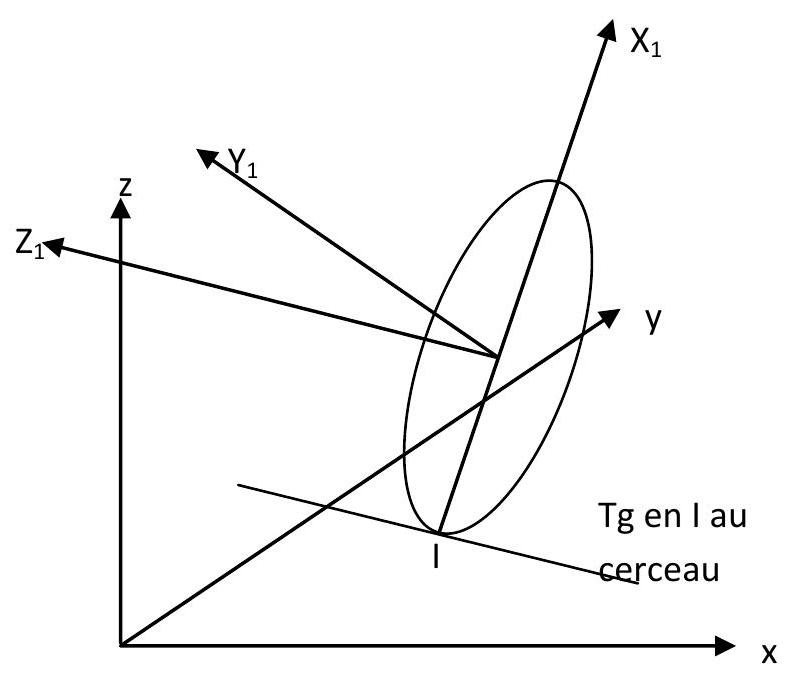
\includegraphics[width=0.55\textwidth]{images/mecanique_solide/ms-003-000.png}\\[4pt]
{\small\itshape Cerceau en contact avec un plan : repère et point de contact $I$.}
\end{center}

\begin{center}
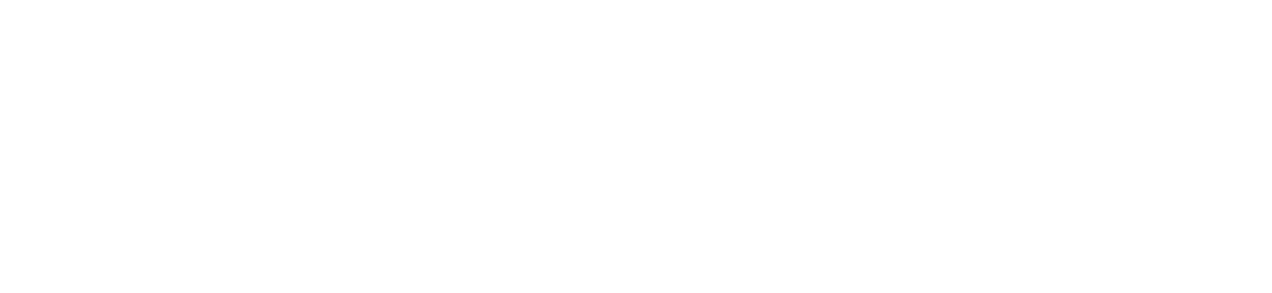
\includegraphics[width=0.50\textwidth]{images/mecanique_solide/ms-006-007.png}\\[4pt]
{\small\itshape Repère $R_1$ en rotation uniforme autour de $Oz_0$ : position du centre $A_1$ et trajectoire circulaire de rayon $R$.}
\end{center}

Le cerceau tourne autour de l'axe $O_1\vec{x}_1$ dans $R_1$ avec une vitesse angulaire $\dot{\varphi}$ :
\[
\vec{\Omega}(C_1/R_1) = \dot{\varphi}\,\vec{x}_1.
\]

Le repère $R_1$ tourne autour de $Oz_0$ à vitesse $\dot{\theta}$ :
\[
\vec{\Omega}(C_1/R_0) = \vec{\Omega}(C_1/R_1) + \vec{\Omega}(R_1/R_0) = \dot{\varphi}\,\vec{x}_1 + \dot{\theta}\,\vec{z}_0.
\]

\textbf{2. Vitesses.}

Le centre $A_1$ du cerceau est à distance $R$ de $O_1$ et suit un mouvement circulaire dans $R_0$ :
\[
\vec{V}(A_1/R_0) = R\dot{\theta}\,\vec{y}_1.
\]

Vitesse du point géométrique de contact $I_{G_1}$ (point de $(\pi)$, donc fixe dans $R_0$... mais $I_{G_1}$ se déplace) :
\[
\vec{V}(I_{G_1}/R_0) = \vec{V}(A_1/R_0) + \vec{\Omega}(C_1/R_0) \wedge \overrightarrow{A_1 I_{G_1}} = R\dot{\theta}\,\vec{y}_1 \quad \Rightarrow \quad \vec{v}(I_{G_1}/R_0) = R\dot{\theta}\,\vec{y}_1.
\]

Vitesse du point matériel $I_1$ appartenant au cerceau :
\[
\vec{V}(I_1/R_0) = \vec{V}(A_1/R_0) + \vec{\Omega}(C_1/R_0) \wedge \overrightarrow{A_1 I_1} = (R\dot{\theta} + a\dot{\varphi})\,\vec{y}_1.
\]

\textbf{3. Condition de roulement sans glissement.}

La condition $\vec{V}(I_1 \in C_1/R_0) = \vec{V}(I_{G_1} \in (\pi)/R_0) = \vec{0}$ (le plan est fixe) donne :
\[
R\dot{\theta} + a\dot{\varphi} = 0 \quad \Rightarrow \quad \dot{\varphi} = -\frac{R}{a}\dot{\theta}.
\]
\end{boitecorrige}

% ----------------------
\begin{boiteexercice}
\textbf{Exercice 6 - Système barre et disque : dynamique plane}\niveau{\difficile}

Un système $(\Sigma)$ est constitué d'une barre $AB$ de longueur $2\ell$, de milieu $G_1$, de masse $m_1$ (solide $S_1$) et d'un disque homogène de centre $C$, de rayon $r$, de masse $m_2$ (solide $S_2$). L'extrémité $A$ de $S_1$ glisse sans frottement sur l'axe $Ox_0$. $S_1$ glisse sur $S_2$ avec un coefficient de frottement $f$. On applique sur $S_2$ un couple $\vec{\Gamma} = -\Gamma\,\vec{k}_0$ ($\Gamma > 0$). La position de $S_1$ est repérée par $(x_A, \varphi)$ et celle de $S_2$ par $(x_C, \theta)$.

\begin{enumerate}
  \item Exprimer $\vec{\Omega}(S_1/R_0)$, $\vec{\Omega}(S_2/R_0)$, $\vec{V}(G_1/R_0)$ et $\vec{\gamma}(C/R_0)$.
  \item Donner la condition de roulement sans glissement de $S_2$ sur $Ox_0$.
  \item Appliquer le théorème du centre de masse à $S_1$ et à $S_2$.
\end{enumerate}
\end{boiteexercice}

\begin{boitecorrige}
\textbf{1. Cinématique.}

\begin{center}
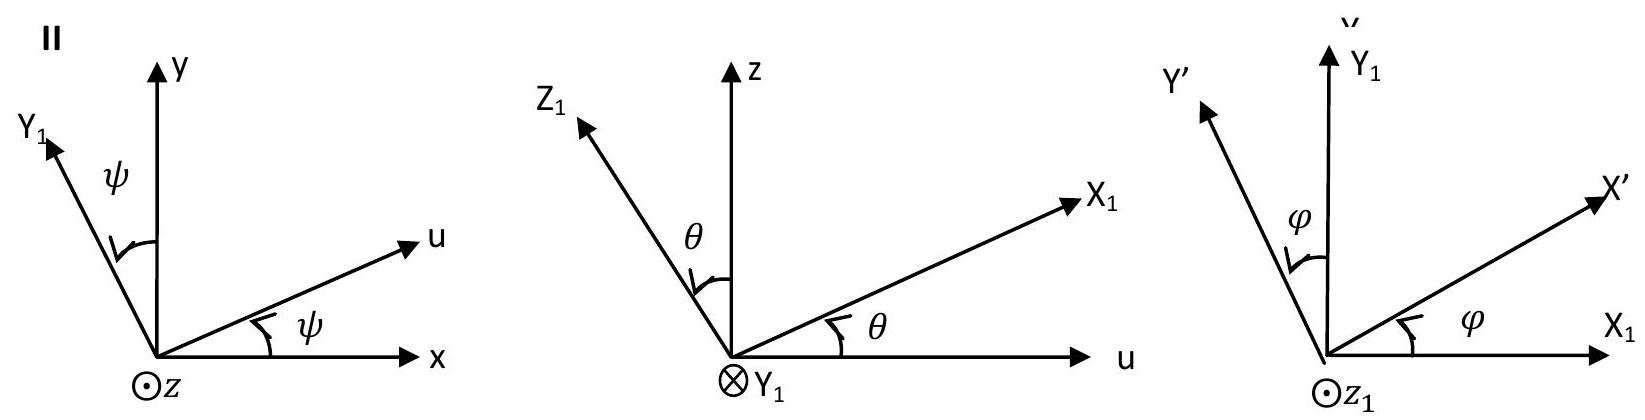
\includegraphics[width=0.45\textwidth]{images/mecanique_solide/ms-004-001.png}\quad
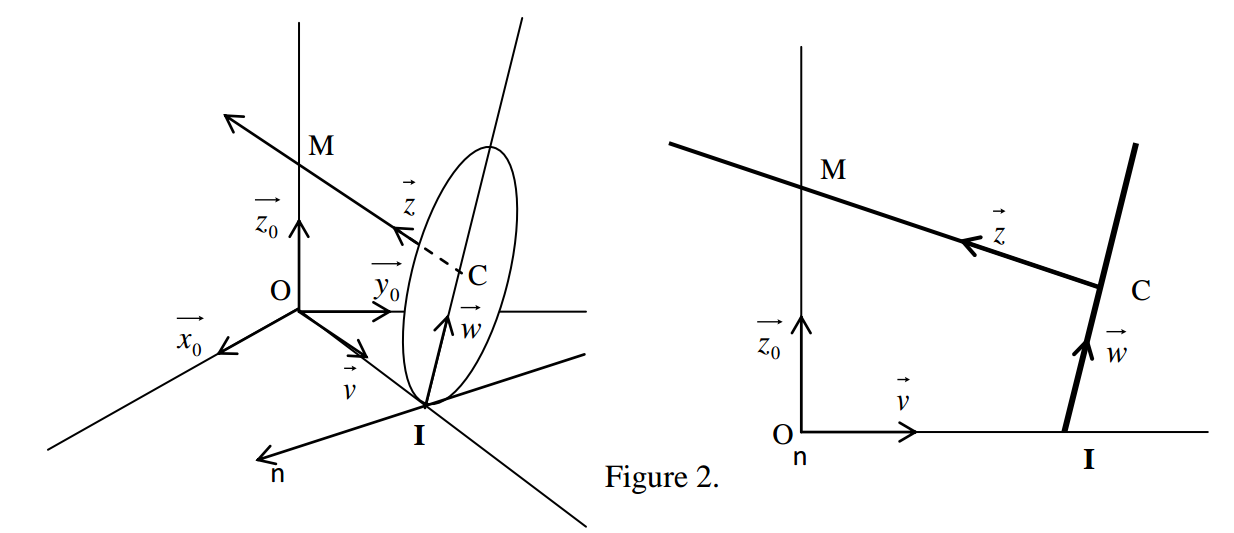
\includegraphics[width=0.45\textwidth]{images/mecanique_solide/ms-005-002.png}\\[4pt]
{\small\itshape Repères d'Euler $(\psi,\theta,\varphi)$ et configuration du système barre--disque (points $O, I, M, C$).}
\end{center}

\begin{center}
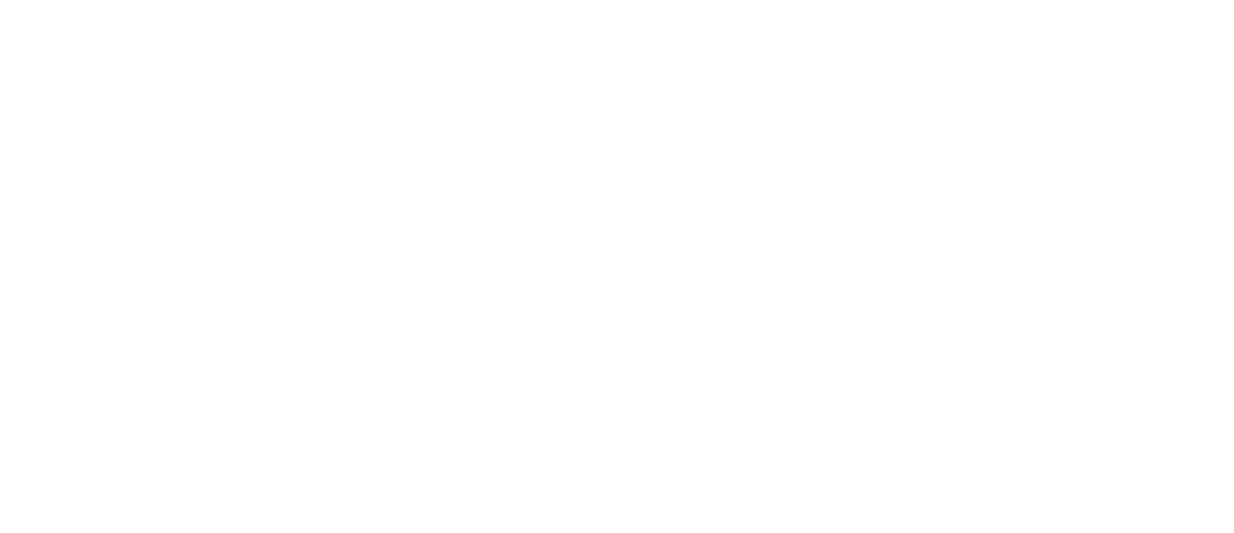
\includegraphics[width=0.50\textwidth]{images/mecanique_solide/ms-005-003.png}\\[4pt]
{\small\itshape Schéma complémentaire : repérage angulaire et points caractéristiques du système barre--disque en dynamique plane.}
\end{center}

\[
\vec{\Omega}(S_1/R_0) = \dot{\varphi}\,\vec{k}_0, \qquad \vec{\Omega}(S_2/R_0) = \dot{\theta}\,\vec{k}_0.
\]

Le milieu $G_1$ de $AB$ a pour coordonnées $(x_A + \ell\cos\varphi,\, \ell\sin\varphi, 0)$. Sa vitesse est :
\[
\vec{V}(G_1/R_0) = (\dot{x}_A - \ell\dot{\varphi}\sin\varphi)\,\vec{i}_0 + (\ell\dot{\varphi}\cos\varphi)\,\vec{j}_0.
\]

L'accélération du centre $C$ du disque (mouvement de translation si $S_2$ roule sans glisser) :
\[
\vec{\gamma}(C/R_0) = \ddot{x}_C\,\vec{i}_0 \quad \text{(si roulement pur sur } Ox_0\text{)}.
\]

\textbf{2. Condition de roulement sans glissement.}

Si $S_2$ roule sans glisser sur $Ox_0$, la vitesse du point de contact de $S_2$ avec l'axe est nulle :
\[
\vec{V}(I \in S_2/R_0) = \vec{V}(C/R_0) + \vec{\Omega}(S_2/R_0) \wedge \overrightarrow{CI} = \vec{0}.
\]
Avec $\overrightarrow{CI} = -r\vec{j}_0$ : $\dot{x}_C\vec{i}_0 + \dot{\theta}\vec{k}_0 \wedge (-r\vec{j}_0) = \dot{x}_C\vec{i}_0 + r\dot{\theta}\vec{i}_0 = \vec{0}$, soit $\dot{x}_C = -r\dot{\theta}$.

\textbf{3. Théorème du centre de masse.}

Pour $S_1$ (projection sur $\vec{i}_0$ et $\vec{j}_0$, avec $\vec{R}_A = R_A\vec{j}_0$ la réaction sur $A$, et $\vec{R}_J = T_j\vec{i}_1 + N_j\vec{j}_1$ la réaction de $S_2$ sur $S_1$) :
\[
m_1\ddot{x}_{G_1} = (T_j\cos\varphi - N_j\sin\varphi), \qquad
m_1\ddot{y}_{G_1} = R_A + T_j\sin\varphi + N_j\cos\varphi - m_1 g.
\]

Pour $S_2$ (translation du centre $C$, forces : réaction $\vec{R}_I$ de $Ox_0$ sur $S_2$, réaction de $S_1$ sur $S_2$ $= -\vec{R}_J$, poids $-m_2 g\vec{j}_0$) :
\[
m_2\ddot{x}_C = -T_j\cos\varphi + N_j\sin\varphi + T_i, \qquad
0 = -T_j\sin\varphi - N_j\cos\varphi + N_i - m_2 g.
\]

Le théorème du moment cinétique en $C$ pour $S_2$ :
\[
\frac{m_2 r^2}{2}\,\ddot{\theta} = r T_i - \Gamma + r(-T_j\cos\varphi + N_j\sin\varphi).
\]
\end{boitecorrige}

\subsection*{Exercice 7 - Cerceau roulant sur un plan horizontal \niveau{\difficile}}

\begin{boiteexercice}
Un cerceau $(C_1)$ de rayon $a$, dans un plan vertical, roule sans glisser sur le plan horizontal $(\pi)$. Le point de contact décrit un cercle de rayon $R$ avec vitesse angulaire uniforme $\dot{\theta} = \mathrm{cte}$. On note $R_0(O,\vec{i}_0,\vec{j}_0,\vec{k}_0)$ le repère fixe et $R_1(O_1,\vec{i}_1,\vec{j}_1,\vec{k}_0)$ le repère en rotation autour de $O\vec{k}_0$.
\begin{enumerate}
  \item Déterminer $\vec{\Omega}(C_1/R_1)$ et $\vec{\Omega}(C_1/R_0)$.
  \item Calculer $\vec{v}(I_{G_1}/R_0)$ et $\vec{v}(I_1/R_0)$. En déduire la condition de roulement sans glissement.
  \item Calculer $\vec{\gamma}(I_{G_1}/R_0)$ et $\vec{\gamma}(I_1/R_0)$.
\end{enumerate}
\end{boiteexercice}

\begin{boitecorrige}
\textbf{1.} Le cerceau tourne autour de $O_1\vec{i}_1$ dans $R_1$ et $R_1$ tourne autour de $O\vec{k}_0$ :
\[
\vec{\Omega}(C_1/R_1) = \dot{\varphi}\,\vec{i}_1 \qquad \vec{\Omega}(C_1/R_0) = \dot{\varphi}\,\vec{i}_1 + \dot{\theta}\,\vec{k}_0
\]

\textbf{2.} Le centre $A_1$ est à distance $R$ de $O$ dans le plan horizontal. La vitesse du point géométrique de contact $I_{G_1}$ (point de $\pi$ projeté) :
\[
\vec{v}(I_{G_1}/R_0) = R\dot{\theta}\,\vec{j}_1
\]
La vitesse du point matériel $I_1 \in C_1$ au contact :
\[
\vec{v}(I_1/R_0) = \vec{v}(A_1/R_0) + \vec{\Omega}(C_1/R_0)\wedge\overrightarrow{A_1I_1} = R\dot{\theta}\,\vec{j}_1 + (\dot{\varphi}\,\vec{i}_1+\dot{\theta}\,\vec{k}_0)\wedge(-a\vec{k}_0) = (R\dot{\theta}+a\dot{\varphi})\,\vec{j}_1
\]
La condition de roulement sans glissement $\vec{v}(I_1/R_0) = \vec{v}(I_{G_1}/R_0)$ donne :
\[
\boxed{R\dot{\theta} + a\dot{\varphi} = 0 \quad\Rightarrow\quad \dot{\varphi} = -\frac{R\dot{\theta}}{a}}
\]

\textbf{3.}
\[
\vec{\gamma}(I_{G_1}/R_0) = -R\dot{\theta}^2\,\vec{i}_1 \qquad \vec{\gamma}(I_1/R_0) = -R\dot{\theta}^2\,\vec{i}_1 + \frac{R^2\dot{\theta}^2}{a}\,\vec{k}_0
\]
\end{boitecorrige}

\subsection*{Exercice 8 - Disque sur barre en rotation \niveau{\difficile}}

\begin{boiteexercice}
$R_0(O,\vec{i}_0,\vec{j}_0,\vec{k}_0)$ est un repère fixe. $S_1$ est une barre $OA$ homogène tournant dans le plan horizontal $(O,\vec{i}_0,\vec{j}_0)$ à la vitesse angulaire $\omega = \dot{\psi}$ autour de $(O,\vec{k}_0)$. $S_2$ est un disque homogène de rayon $R$, de centre $C$, assujetti à rouler sans glisser sur $S_1$ dans le plan vertical $(O,\vec{i}_1,\vec{k}_0)$. On pose $\overrightarrow{OC} = R\vec{k}_0 + x\vec{i}_1$. $R_1$ est lié à $S_1$, $R_2$ est lié à $S_2$.
\begin{enumerate}
  \item Donner $\vec{\Omega}(S_1/R_0)$, $\vec{\Omega}(S_2/R_1)$ et en déduire $\vec{\Omega}(S_2/R_0)$.
  \item Calculer $\vec{v}(I_1\in S_1/R_0)$ et $\vec{v}(I_2\in S_2/R_0)$ où $I$ est le point de contact. En déduire la condition de roulement sans glissement.
  \item Le mouvement de $S_2$ est-il plan dans $R_0$ ?
\end{enumerate}
\end{boiteexercice}

\begin{boitecorrige}
\textbf{1.}
\[
\vec{\Omega}(S_1/R_0) = \dot{\psi}\,\vec{k}_0 \qquad \vec{\Omega}(S_2/R_1) = \dot{\theta}\,\vec{j}_1
\]
\[
\vec{\Omega}(S_2/R_0) = \vec{\Omega}(S_2/R_1) + \vec{\Omega}(R_1/R_0) = \dot{\theta}\,\vec{j}_1 + \dot{\psi}\,\vec{k}_0
\]

\textbf{2.} Point de contact $I$ sur $S_1$ : $\overrightarrow{OI} = x\vec{i}_1$.
\[
\vec{v}(I_1\in S_1/R_0) = \vec{\Omega}(S_1/R_0)\wedge\overrightarrow{OI} = \dot{\psi}\vec{k}_0\wedge x\vec{i}_1 = x\dot{\psi}\,\vec{j}_1
\]
Point $I$ sur $S_2$ : $\overrightarrow{CI} = -R\vec{k}_0$.
\[
\vec{v}(I_2\in S_2/R_0) = \vec{v}(C/R_0) + \vec{\Omega}(S_2/R_0)\wedge\overrightarrow{CI} = (\dot{x}\vec{i}_1 + x\dot{\psi}\vec{j}_1) + (\dot{\theta}\vec{j}_1+\dot{\psi}\vec{k}_0)\wedge(-R\vec{k}_0)
\]
\[
= \dot{x}\vec{i}_1 + x\dot{\psi}\vec{j}_1 + R\dot{\theta}\vec{i}_1 \cdot (-1) = (\dot{x}-R\dot{\theta})\vec{i}_1 + x\dot{\psi}\vec{j}_1
\]
Condition de roulement sans glissement ($\vec{v}(I_1)=\vec{v}(I_2)$ dans $R_0$) :
\[
\boxed{\dot{x} = R\dot{\theta}}
\]

\textbf{3.} $\vec{\Omega}(S_2/R_0) = \dot{\theta}\vec{j}_1 + \dot{\psi}\vec{k}_0$ a deux composantes : le mouvement de $S_2$ n'est \textbf{pas plan} dans $R_0$ (il est plan dans $R_1$).
\end{boitecorrige}

\subsection*{Exercice 9 - Disque sur tapis roulant incliné \niveau{\difficile}}

\begin{boiteexercice}
Un disque homogène de masse $m$, de rayon $r$, est posé sans vitesse initiale sur un tapis roulant incliné d'un angle $\alpha$. Le tapis se déplace à la vitesse $v_0\vec{i}_0$ (vers le haut). Le coefficient de frottement cinétique est $f$. La réaction du tapis est $\vec{R} = T\vec{i}_0 + N\vec{j}_0$ avec $|T| = fN$.
\begin{enumerate}
  \item Calculer la vitesse de glissement initiale du disque sur le tapis.
  \item Appliquer le P.F.D. et le théorème du moment cinétique en $G$ pour obtenir $\ddot{x}_C$ et $\ddot{\theta}$.
  \item Montrer que $\dot{v}_g = 3gf\cos\alpha - g\sin\alpha$ (si le glissement a lieu vers le bas).
  \item Décrire qualitativement l'évolution du glissement.
\end{enumerate}
\end{boiteexercice}

\begin{boitecorrige}
\textbf{1.} À $t=0$, $\dot{x}_C = 0$ et $\dot{\theta} = 0$. La vitesse de glissement est $\vec{v}_g = \vec{v}(I\in\text{disque}) - \vec{v}(I\in\text{tapis}) = (0 + 0 - v_0)\vec{i}_0$, soit :
\[
\vec{v}_{g0} = -v_0\,\vec{i}_0
\]
Le disque glisse vers le bas par rapport au tapis ($v_g < 0$), donc $T = +fN\vec{i}_0 = fmg\cos\alpha\,\vec{i}_0$.

\textbf{2.} Théorème du centre de masse (axe $x$) : $m\ddot{x}_C = T - mg\sin\alpha = fmg\cos\alpha - mg\sin\alpha$.

Théorème du moment cinétique en $G$ : $I_G\ddot{\theta} = \frac{mr^2}{2}\ddot{\theta} = rT = rfmg\cos\alpha$, d'où $\ddot{\theta} = 2fg\cos\alpha/r$.

\textbf{3.} $v_g = \dot{x}_C + r\dot{\theta} - v_0$, donc $\dot{v}_g = \ddot{x}_C + r\ddot{\theta}$:
\[
\dot{v}_g = (fg\cos\alpha - g\sin\alpha) + r\cdot\frac{2fg\cos\alpha}{r} = 3fg\cos\alpha - g\sin\alpha
\]

\textbf{4.} Si $f > \tan\alpha/3$ : $\dot{v}_g > 0$, le glissement diminue ($v_g$ part de $-v_0$ et tend vers $0$) : il y a d'abord glissement puis roulement pur.

Si $f < \tan\alpha/3$ : $\dot{v}_g < 0$, le glissement augmente en valeur absolue : le disque continue à glisser indéfiniment.
\end{boitecorrige}

\subsection*{Exercice 10 - Pendule double : équations de Lagrange \niveau{\difficile}}

\begin{boiteexercice}
Un pendule double plan est constitué de deux masses ponctuelles $m_1$ et $m_2$, reliées par des tiges rigides de longueurs $\ell_1$ et $\ell_2$. Les angles $\theta_1$ et $\theta_2$ repèrent les positions par rapport à la verticale.
\begin{enumerate}
  \item Exprimer les positions des deux masses en coordonnées cartésiennes.
  \item Calculer l'énergie cinétique $T$ du système.
  \item Calculer l'énergie potentielle $V$ du système.
  \item Pour les petites oscillations, linéariser les équations de Lagrange.
\end{enumerate}
\end{boiteexercice}

\begin{boitecorrige}
\textbf{1.} Positions :
\[
\vec{r}_1 = \ell_1(\sin\theta_1,-\cos\theta_1) \qquad \vec{r}_2 = \vec{r}_1 + \ell_2(\sin\theta_2,-\cos\theta_2)
\]

\textbf{2.} Vitesses :
\[
\dot{\vec{r}}_1 = \ell_1\dot{\theta}_1(\cos\theta_1,\sin\theta_1)
\]
\[
\dot{\vec{r}}_2 = \ell_1\dot{\theta}_1(\cos\theta_1,\sin\theta_1) + \ell_2\dot{\theta}_2(\cos\theta_2,\sin\theta_2)
\]
\[
T = \frac{1}{2}m_1\ell_1^2\dot{\theta}_1^2 + \frac{1}{2}m_2\!\left[\ell_1^2\dot{\theta}_1^2 + \ell_2^2\dot{\theta}_2^2 + 2\ell_1\ell_2\dot{\theta}_1\dot{\theta}_2\cos(\theta_1-\theta_2)\right]
\]

\textbf{3.}
\[
V = -m_1g\ell_1\cos\theta_1 - m_2g(\ell_1\cos\theta_1+\ell_2\cos\theta_2)
\]

\textbf{4.} Pour les petites oscillations ($\sin\theta\approx\theta$, $\cos\theta\approx1$, $\cos(\theta_1-\theta_2)\approx1$) :
\[
(m_1+m_2)\ell_1\ddot{\theta}_1 + m_2\ell_2\ddot{\theta}_2 + (m_1+m_2)g\theta_1 = 0
\]
\[
m_2\ell_2\ddot{\theta}_2 + m_2\ell_1\ddot{\theta}_1 + m_2 g\theta_2 = 0
\]
Ce système de deux équations couplées admet des solutions oscillatoires de deux fréquences propres distinctes.
\end{boitecorrige}


\subsection*{Exercice 11 - Barre glissante et disque en contact \niveau{\difficile}}

\begin{boiteexercice}
On considère un système $(\Sigma)$ de deux solides $(S_1)$ et $(S_2)$. Le solide $(S_1)$ est une barre $AB$ de longueur $2\ell$, de milieu $G$ et de masse $m_1$ ; $(S_2)$ est un disque homogène de centre $C$, de rayon $r$ et de masse $m_2$. L'extrémité $A$ de $(S_1)$ glisse sans frottement sur l'axe $Ox_0$ ; $(S_2)$ est en contact avec $(S_1)$ en $J$ (avec coefficient de frottement $f$, glissement). Un couple $\vec{\Gamma} = -\Gamma\,\vec{k}_0$ ($\Gamma>0$) est appliqué à $(S_2)$.

\begin{enumerate}
  \item[\textbf{a)}] Exprimer $\vec{\Omega}(S_i/R_0)$, $\vec{v}(G/R_0)$, $\vec{\gamma}(G/R_0)$ et $\vec{\gamma}(C/R_0)$. Donner la condition de roulement sans glissement de $(S_2)$ sur $Ox_0$.
  \item[\textbf{b)}] Sachant que $\tan(\varphi/2) = r/(x_C - x_A)$, montrer que la vitesse de glissement de $(S_1)$ sur $(S_2)$ est $\vec{v}_g = [(x_A-x_C)\cos\varphi - r\dot\theta]\,\vec{j}_1$.
  \item[\textbf{c)}] Calculer les moments cinétique et dynamique de chaque solide. En déduire les équations du mouvement.
\end{enumerate}
\end{boiteexercice}

\begin{boitecorrige}
\begin{center}
  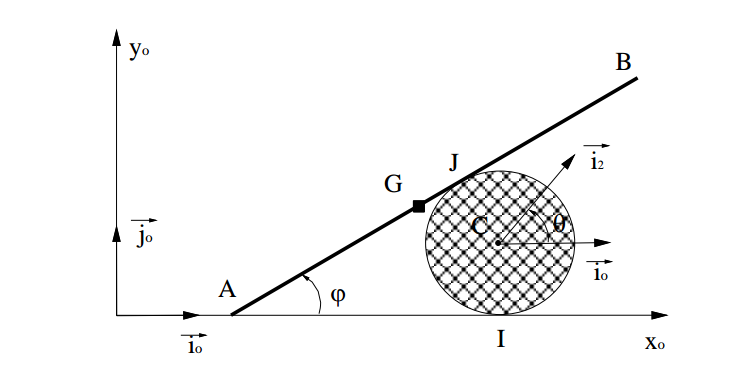
\includegraphics[width=0.85\textwidth]{images/im103.png}
\end{center}

La résolution complète conduit aux schémas suivants :

\begin{center}
  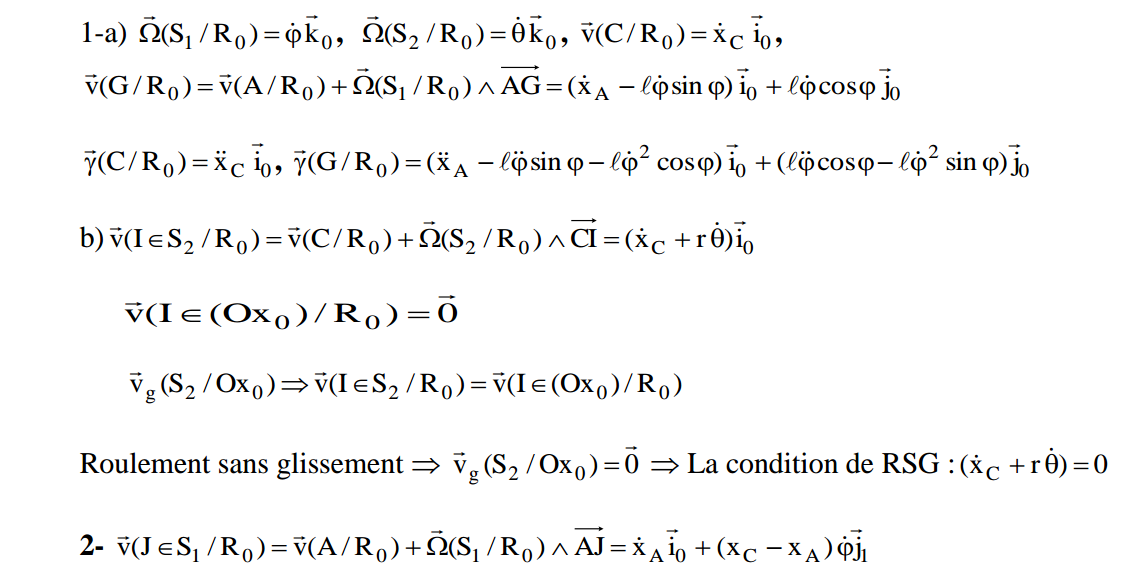
\includegraphics[width=0.85\textwidth]{images/im104.png}
\end{center}
\begin{center}
  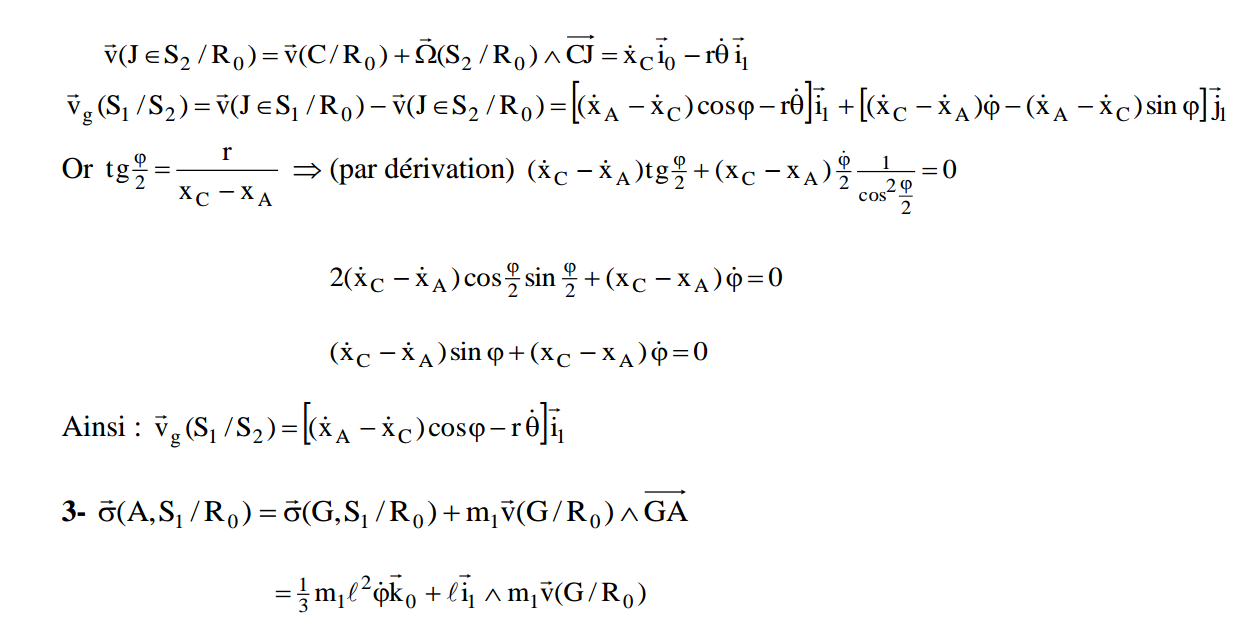
\includegraphics[width=0.85\textwidth]{images/im106.png}
\end{center}
\begin{center}
  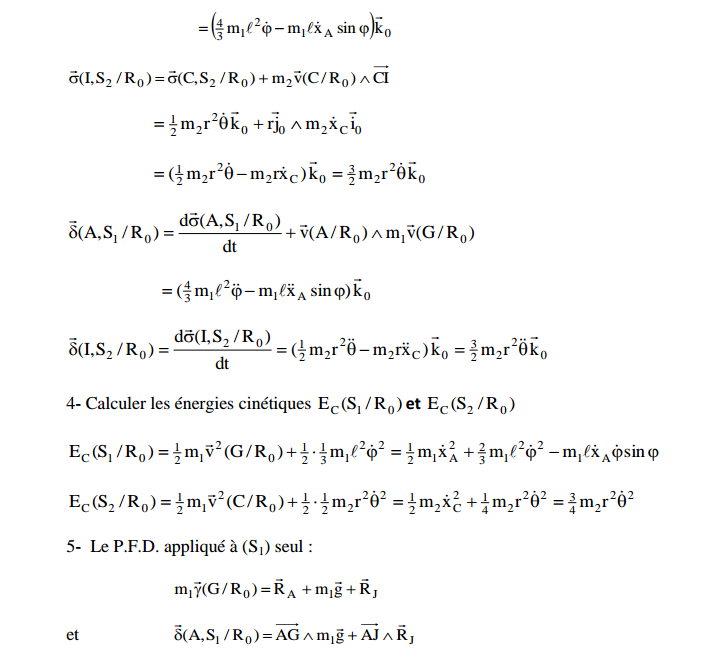
\includegraphics[width=0.85\textwidth]{images/im107.png}
\end{center}

\textbf{Éléments clés de la résolution :}

\textbf{1. Cinématique.}
\[
\vec{\Omega}(S_1/R_0) = \dot\varphi\,\vec{k}_0, \qquad
\vec{\Omega}(S_2/R_0) = \dot\theta\,\vec{k}_0.
\]
\[
\vec{v}(G/R_0) = \dot x_A\,\vec{i}_0 + \ell\dot\varphi\,\vec{j}_1.
\]

Condition de roulement sans glissement de $(S_2)$ sur $Ox_0$ :
\[
\vec{v}(I\in S_2/R_0) = \vec{0} \implies \dot x_C = r\dot\theta.
\]

\textbf{2. Application du P.F.D.}
En appliquant le P.F.D.\ à $(S_1)$ seul (théorème du centre de masse + moment en $A$) et à $(S_2)$ seul (théorème du centre de masse + moment en $C$), on obtient 6 équations scalaires pour les 8 inconnues
\[
(x_A,\, x_C,\, \varphi,\, \theta,\, R_A,\, T_J,\, T_I,\, N_I).
\]
Les liaisons géométriques de contact fournissent les 2 équations manquantes.
\end{boitecorrige}

\ifdefined\inMainDoc\else\end{document}\fi
